\documentclass{article}
\usepackage[utf8]{inputenc}
\usepackage{amsmath}
\usepackage{geometry}
 \geometry{
 a4paper,
 total={170mm,257mm},
 left=10mm,
 top=15mm,
 right=10mm,
 bottom=15mm
 }
 
\usepackage{comment} % enables the use of multi-line comments (\ifx \fi) 
\usepackage{graphicx}
\usepackage{subfig}
\usepackage{etoolbox}

\BeforeBeginEnvironment{figure}{\vskip-2ex}
\AfterEndEnvironment{figure}{\vskip-2ex}


\begin{document}
%Header-Make sure you update this information!!!!
\noindent\large\textbf{ED5330} \hfill \textbf{Divyanshu Pundir} \\
\large\textbf{Control of Automotive Systems} \hfill \textbf{ED15013} \\
\\
\large\textbf{Brake System Modelling and Control Report}\\


\section*{Problem Statement}
To determine the transfer function of air brake system consisting of electro-pneumatic regulator (EPR).

\section{Check for Linear Time Invariant System/Spectral Analysis}
Sine sweep test is done to check whether the system is LTI or not.
When a sinusoidal system is given to an LTI system, the output is another sinusoid with the same frequency as that of the input, but it is scaled and has some phase difference.

On taking FFT for the input and output, it is seen that for all (but one) inputs, the dominant frequency is same for both input and output.
Fourier transform represents a time domain signal as a frequency domain signal, i.e., it breaks up a signal into the frequencies it is composed of.
Magnitude plot of FFT of an ideal sinusoid has two impulse whose magnitude is half its amplitude, and they are present at positive and negative value of the frequency of the sinusoid.
Hence, it is assumed that the dominant frequency is the frequency of the sinusoid and the rest is noise. Since, the dominant frequency of both the input and output is same for a number of different pairs, it can be concluded that the system is LTI.

After this, the gain is calculated for different frequencies and a Bode plot is created using these.

\begin{figure}[h]%
    \centering
    \subfloat{{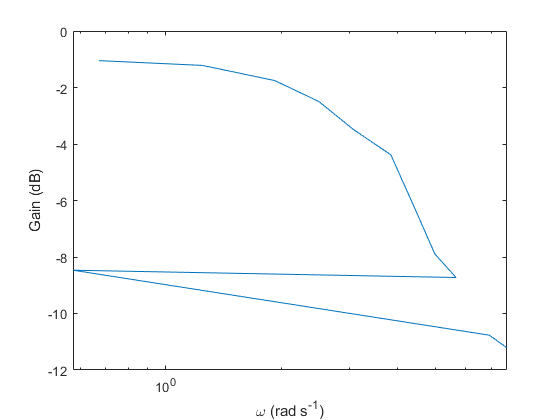
\includegraphics[width=7cm]{images/spectral_outlier.png} }}%
    \qquad
    \subfloat{{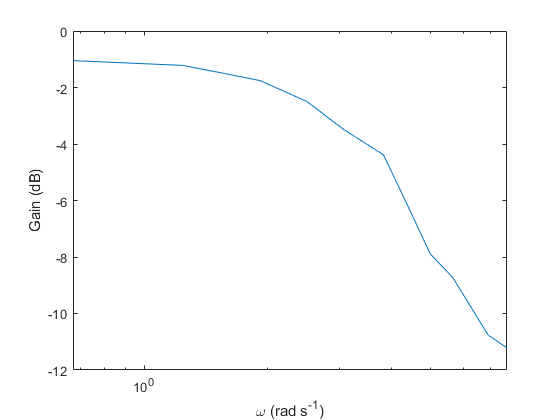
\includegraphics[width=7cm]{images/spectral.png} }}%
    \caption{Bode Plot}%
    \label{fig:bode}%
\end{figure}

Left figure is the Bode plot created using the actual data. It is assumed that one point is a outlier and hence it is ignored. The right plot is the one obtained after ignoring the outlier.

The slope is calculated for the higher frequencies and the value comes out to be \textbf{\textit{-22.7110 dB/decade}}
For low frequencies, the slope can be assumed to be close to \textbf{\textit{0}}
Since the plot does not start from 0, there is a constant steady state gain.

On taking time delay into consideration, the plant transfer function is as follows:
\[P(s) = \frac{K}{1 + \tau s} e^{-T_d s}\]

After using Pade’s approximation:
\[P(s) = \frac{K(2 - T_d s)}{(1 + \tau s)(2 + T_d s)}\]


\section{Parameter Estimation/Step Input Analysis}
Step response data is used to determine the parameters.

\subsection{Steady State Gain (K)}
Ratio of steady state value of output to that of input is taken. Average of values obtained from different inputs is finally used

\subsection{Time Delay ($T_d$)}
The time difference from the start and at the point which the output starts becoming more than 0.005 is taken.

\subsection{Time Constant ($\tau$)}
The time difference from the point which the output starts becoming more than \textbf{\textit{0.005}} to the point at which the output becomes equals to 0.632 times its steady state value is taken.

But the variation in tau values for different equations is considerable. Therefore, the system is simulated between a range of values of tau and the one which gives the least \textbf{MAPE} is taken.

\[MAPE = \frac{1}{N} \sum \frac{simulated \; value - experimental \; value}{experimental \; value} \times 100\]

\begin{table}[h]
\begin{center}
\captionof{table}{MAPE values}
\begin{tabular}{|l|l|l|l|l|l|l|l|}
\hline
$\tau$  &  & MAPE S\_5   & MAPE S\_6   & MAPE S\_7   & MAPE S\_8   &  & Avg. MAPE   \\ \hline
    %  &  &             &             &             &             &  &             \\ \hline
    \hline
0.4  &  & 3.867663051 & 3.781248034 & 4.691096652 & 2.405167392 &  & 3.686293782 \\ \hline
0.42 &  & 3.808216534 & 3.469758609 & 4.038229457 & 2.161618411 &  & 3.369455753 \\ \hline
0.44 &  & 3.849628439 & 3.270478747 & 3.467499642 & 2.091418968 &  & 3.169756449 \\ \hline
0.46 &  & 3.979895638 & 3.190727053 & 2.979511847 & 2.221582413 &  & 3.092929238 \\ \hline
0.48 &  & 4.181915622 & 3.219945278 & 2.581137661 & 2.480255865 &  & 3.115813607 \\ \hline
0.5  &  & 4.437405934 & 3.335479594 & 2.30373004  & 2.828297891 &  & 3.226228365 \\ \hline
0.52 &  & 4.732945559 & 3.550329189 & 2.185721771 & 3.239582963 &  & 3.42714487  \\ \hline
0.54 &  & 5.065253351 & 3.83450016  & 2.234566812 & 3.702916045 &  & 3.709309092 \\ \hline

\end{tabular}
\end{center}
\end{table}

\subsection{Calculated Values}
$K = 0.90035 \; bar/V$\\
$T_d = 0.035 \; s$\\
$\tau = 0.46 \; s$


\section{Controller Design}
For a closed loop system:
\[G(s) = C(s)P(s)\]
\[\frac{Y(s)}{R(s)} = \frac{G(s)}{1 + G(s)H(s)}\]

For unity negative feedback $H(s) = 1$

\subsection{Performance Criteria}
\subsubsection{Maximum Peak Overshoot $\leq 10 \%$}

\[e^{\frac{-\zeta \pi}{\sqrt{1 - \zeta^2}}} \leq 0.1 \;\; \Rightarrow \;\; \zeta \geq 0.5910 \;\; \Rightarrow \;\; \beta \leq 53.77\]

Since, 
\[ \zeta = \cos{\beta}\]

\subsubsection{Rise Time $\leq 0.7 \; s$}
\[\frac{\pi - \beta}{\omega_d} \leq 0.7 \;\; \Rightarrow \;\; \omega_d \geq \frac{\pi - \beta}{0.7}\]

$\omega_d$ gives the imaginary part of the pole. For each $\beta$ we will get a range for $\omega_d$. If $\beta$ = 0, then we will get the \textit{greatest} lower-bound for $\omega$ which will satisfy performance for all values of $\beta$.

Hence, $\omega_d \geq \frac{\pi}{0.7} = 4.488$

\subsection{P - Controller}

\[C(s) = K_p\]
\[Open \; Loop \; Transfer \; Function = G(s)H(s) = \frac{K_p K(2 - T_d s)}{(1 + \tau s)(2 + T_d s)}\]

\subsubsection{Stability Criteria}
For stability, the roots closed loop characteristic equation should lie on the Right Half Plane

\[ 1 + G(s)H(s) = 0\]
\[s^2 + (59.32 - 1.96K_p)s + (124.22 + 111.84 K_p) = 0\]

According to Routh's criteria, coefficients of $s^2$ and $s$, and constant should be greater than zero. Therefore we get:

\[ -1.11 < K_p < 30.26\]

\subsubsection{Root Locus and Output}
On plotting the root locus for the closed loop system the range of value of $K_p \in [4.7, 9.3]$
These values satisfy stability.
Out of these values $K_p = 9.3$ gives the least steady state error of $10.67 \%$ and an $MP = 9.32 \%$


\subsection{PD - Controller}
\[C(s) = K_p + s K_d\]
\[Open \; Loop \; Transfer \; Function = G(s)H(s) = \frac{(K_p + s K_d)K(2 - T_d s)}{(1 + \tau s)(2 + T_d s)}\]

\subsubsection{Stability Criteria}
\[(1-1.96K_d)s^2 + (111.84K_d - 1.96K_p + 59.32)s + (124.22 + 111.84 K_p) = 0\]
                      
Using Routh's criteria
\[ K_p > -1.11 \;\;\;\; and \;\;\;\; K_d < 0.51\]

\subsubsection{Root Locus and Output}
The ratio of $\frac{K_d}{K_p}$ is taken to be 0.01\\
From root locus - $K_p \in [6.6,15.5]$ out of which $K_p = 15.5$ gave the least steady state error and $MP = 9.86 \%$.

\subsection{PI - Controller}
\[C(s) = K_p + \frac{K_i}{s}\]
\[Open \; Loop \; Transfer \; Function = G(s)H(s) = \frac{(K_p + \frac{K_i}{s})K(2 - T_d s)}{(1 + \tau s)(2 + T_d s)}\]

\subsubsection{Stability Criteria}
\[s^3 + (59.32 - 1.96K_p)s^2 + (111.84K_p - 1.96K_i + 124.22)s + (111.84K_i) = 0\]

Using Routh's criteria
\[ K_p < 30.26 \;\;\;\; and \;\;\;\; K_i > 0\]

\subsubsection{Root Locus and Output}
The ratio $\frac{K_i}{K_p}$ is taken to be $\frac{1}{\tau}$ as this results in cancellation of an open loop pole. The open loop transfer function thus becomes
\[ \frac{K_p K(2 - T_d s)}{\tau s(2 + T_d s)}\]
From root locus $K_p \in [5.7,9.4]$. $K_p = 6.2$ is chosen as it gives optimal rise time and maximum peak overshoot.


\subsection{PID - Controller}
\[C(s) = K_p + s K_d+ \frac{K_i}{s}\]
\[Open \; Loop \; Transfer \; Function = G(s)H(s) = \frac{(K_p + s K_d + \frac{K_i}{s})K(2 - T_d s)}{(1 + \tau s)(2 + T_d s)}\]

\subsubsection{Stability Criteria}
\[(1 - 1.96K_d) s^3 + (111.84K_d - 1.96K_p + 59.32)s^2 + (111.84K_p - 1.9573K_i + 124.22)s + (111.84K_i) = 0\]

Using Routh's criteria
\[ K_d < 0.51 \;\;\;\; and \;\;\;\; K_i > 0\]

\subsubsection{Root Locus and Output}
The ratio $\frac{K_i}{K_p} = \frac{1}{\tau}$ and $\frac{K_d}{K_p} = 0.001$. 
From root locus $K_p \in [5.3,9.8]$. $K_p = 6.0$ is chosen as it gives the least rise time as well as maximum peak overshoot.

\section{Conclusion}
The best values of controller gains for different controllers are given in the table below.

P and PD controller are not chosen as steady state error in this case cannot be avoided if we use these.

Both PI and PID controllers gave \textbf{\textit{zero}} steady state error.
PID controller is chosen as it gave the best performance in terms of least maximum peak overshoot and rise time. Also Initial oscillation is lesser in case of a PID controller.

\begin{table}[h]
\begin{center}
\captionof{table}{Best Controller Gains}
\begin{tabular}{|l|l|l|l|l|}
\hline
Controller Type    &  & Kp (V/bar) & Kd (V s/bar) & Ki (V/(bar s)) \\ \hline
    % &  &            &              &                \\ \hline
    \hline
P   &  & 9.3        & -            & -                \\ \hline
PD  &  & 15.5       & 0.155        & -               \\ \hline
PI  &  & 6.2        & -             & 13.48          \\ \hline
PID &  & 6.0        & 0.006        & 13.04          \\ \hline
\end{tabular}
\end{center}
\end{table}

\newpage
\section{Plots}

\begin{figure}[h]%
    \vspace*{-0.5cm}
    
    \centering
    \subfloat[Root Locus - P]{{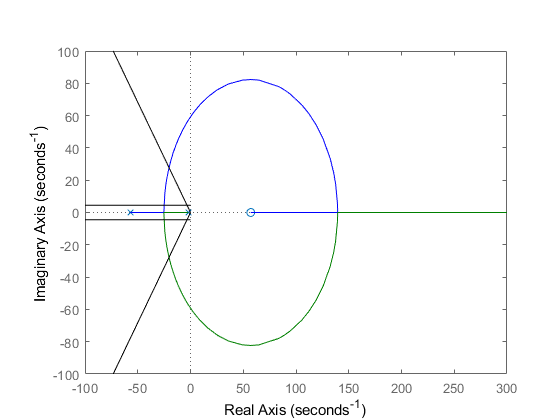
\includegraphics[width=6cm,trim={0.75cm 0cm 1.4cm 0.75cm},clip]{images/r_locus_p.png} }}%
    \qquad
    \subfloat[Output - P]{{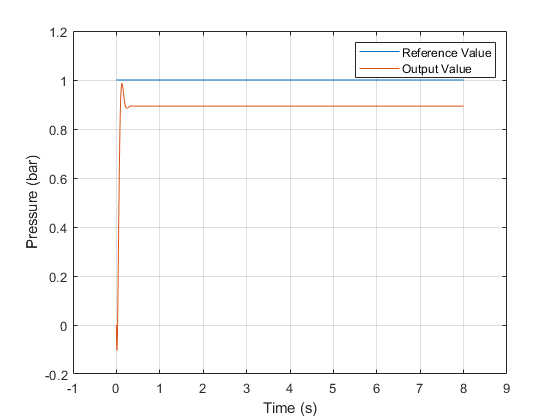
\includegraphics[width=6cm,trim={0.75cm 0cm 1.4cm 0.75cm},clip]{images/output_p.png} }}%
    
    
    \centering
    \subfloat[Root Locus - PD]{{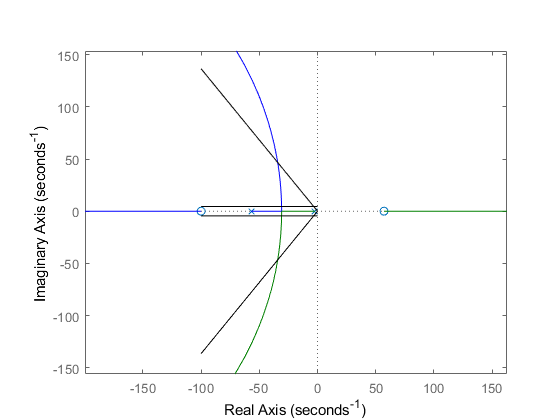
\includegraphics[width=6cm,trim={0.75cm 0cm 1.4cm 0.75cm},clip]{images/r_locus_pd.png} }}%
    \qquad
    \subfloat[Output - PD]{{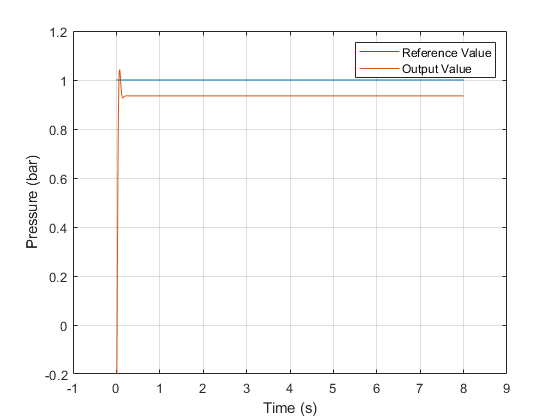
\includegraphics[width=6cm,trim={0.75cm 0cm 1.4cm 0.75cm},clip]{images/output_pd.png} }}%
    
    
    \centering
    \subfloat[Root Locus - PI]{{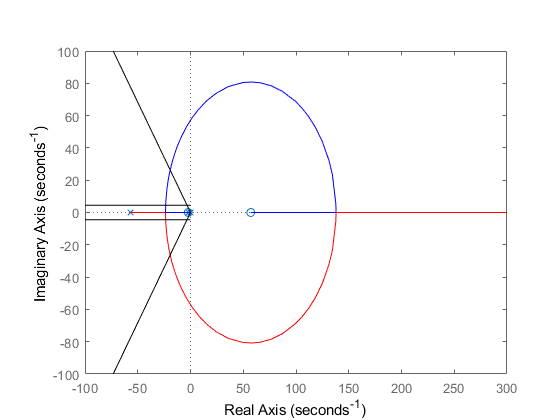
\includegraphics[width=6cm,trim={0.75cm 0cm 1.4cm 0.75cm},clip]{images/r_locus_pi.png} }}%
    \qquad
    \subfloat[Output - PI]{{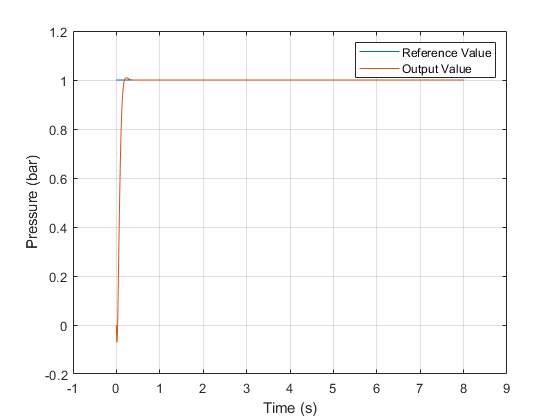
\includegraphics[width=6cm,trim={0.75cm 0cm 1.4cm 0.75cm},clip]{images/output_pi.png} }}%
    
    
    \centering
    \subfloat[Root Locus - PID]{{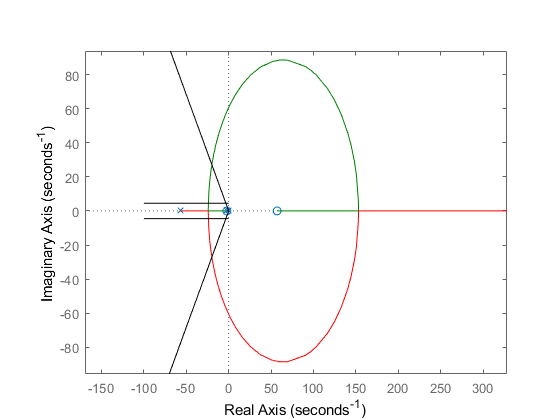
\includegraphics[width=6cm,trim={0.75cm 0cm 1.4cm 0.75cm},clip]{images/r_locus_pid.png} }}%
    \qquad
    \subfloat[Output - PID]{{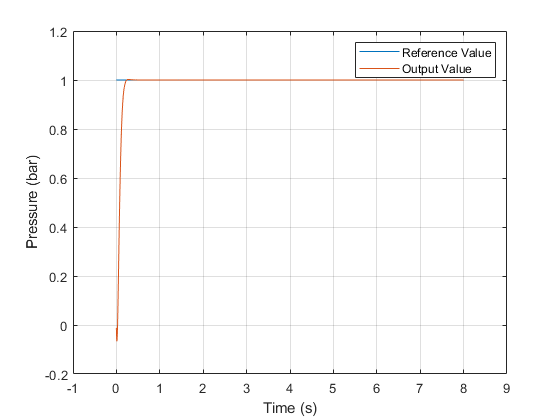
\includegraphics[width=6cm,trim={0.75cm 0cm 1.4cm 0.75cm},clip]{images/output_pid.png} }}%
    
    \vspace*{-1.5cm}
\end{figure}

\end{document}
